\section{Results} \label{results}

% In addition to the randomly generated initial function, I developed the \verb|GenerateHeuristicInitialSolution()|
% which construct the initial solution according to an heuristic which aims to minimize the number of constraint violations.

% The general outline of the algorithm is as follows:
% \begin{enumerate}
%   \item Construct a solution by ordering the solution components in an ascending way according to their time windows closing time
%   \item For a number of times equal to the solution size divided by 10:
%   \begin{enumerate}
%     \item Select a random solution component in the solution
%     \item Select a neighborhood size randomly.
%     \item Shuffle the elements in the chosen neighborhood of the chosen solution
%   \end{enumerate}
% \end{enumerate}

% Due to the lack of time, I was only able to test the heuristic function on a limited number of instances.
% The same metrics as in \ref{subsec:metric} will be used to evaluate the algorithms.

% \subsubsection{n80w200.001}
% \begin{center}
% \includegraphics[width=0.6\textwidth,keepaspectratio]{{II-H/n80w200.001-CpuTime}.pdf}
% \captionof{figure}{n80w200.001 - Runtime boxplots for the different iterative improvement algorithms with heuristic initialization}
% \end{center}

% \begin{center}
% \includegraphics[width=0.6\textwidth,keepaspectratio]{{II-H/n80w200.001-PRPD}.pdf}
% \captionof{figure}{n80w200.001 - PRPD boxplots for the different iterative improvement algorithms with heuristic initialization}
% \end{center}

% \begin{center}
% \begin{tabular}{|l|l|}
% \hline
% \textbf{Test} & \textbf{P-Value} \\
% \hline
% First vs best - Transpose&3.95591160889952e-18\\
% \hline
% First vs best - Exchange&3.95591160889952e-18\\
% \hline
% First vs best - Insert&7.16468868599392e-06\\
% \hline
% Exchange vs Insert - First&3.95591160889952e-18\\
% \hline
% Exchange vs Insert - Best&3.9550194074242e-18\\
% \hline
% \end{tabular}
% \captionof{table}{n80w200.001 - Results of Wilcoxon paired signed rank test}
% \label{tab:w.21}
% \end{center}

% \subsubsection{n80w200.002}
% \begin{center}
% \includegraphics[width=0.6\textwidth,keepaspectratio]{{II-H/n80w200.002-CpuTime}.pdf}
% \captionof{figure}{n80w200.002 - Runtime boxplots for the different iterative improvement algorithms with heuristic initialization}
% \end{center}

% \begin{center}
% \includegraphics[width=0.6\textwidth,keepaspectratio]{{II-H/n80w200.002-PRPD}.pdf}
% \captionof{figure}{n80w200.002 - PRPD boxplots for the different  iterative improvement algorithms with heuristic initialization}
% \end{center}

% \begin{center}
% \begin{tabular}{|l|l|}
% \hline
% \textbf{Test} & \textbf{P-Value} \\
% \hline
% First vs best - Transpose&3.95591160889952e-18\\
% \hline
% First vs best - Exchange&3.95591160889952e-18\\
% \hline
% First vs best - Insert&1.5011633635878e-17\\
% \hline
% Exchange vs Insert - First&3.95591160889952e-18\\
% \hline
% Exchange vs Insert - Best&3.9552424399092e-18\\
% \hline
% \end{tabular}
% \captionof{table}{n80w200.002 - Results of Wilcoxon paired signed rank test}
% \label{tab:w.22}
% \end{center}

% \subsubsection{n80w200.003}
% \begin{center}
% \includegraphics[width=0.6\textwidth,keepaspectratio]{{II-H/n80w200.003-CpuTime}.pdf}
% \captionof{figure}{n80w200.003 - Runtime boxplots for the different iterative improvement algorithms with heuristic initialization}
% \end{center}

% \begin{center}
% \includegraphics[width=0.6\textwidth,keepaspectratio]{{II-H/n80w200.003-PRPD}.pdf}
% \captionof{figure}{n80w200.003 - PRPD boxplots for the different iterative improvement algorithms with heuristic initialization}
% \end{center}

% \begin{center}
% \begin{tabular}{|l|l|}
% \hline
% \textbf{Test} & \textbf{P-Value} \\
% \hline
% First vs best - Transpose&3.95591160889952e-18\\
% \hline
% First vs best - Exchange&3.95591160889952e-18\\
% \hline
% First vs best - Insert&2.88431649979563e-16\\
% \hline
% Exchange vs Insert - First&3.9556885406462e-18\\
% \hline
% Exchange vs Insert - Best&4.33074349739998e-18\\
% \hline
% \end{tabular}
% \captionof{table}{n80w200.003 - Results of Wilcoxon paired signed rank test}
% \label{tab:w.23}
% \end{center}

% \subsection{Statistics}

% \subsubsection{Transpose-First Improvement}
% \begin{center}
% \begin{tabular}{|l|c|l|l|}
% \hline
% \textbf{Instance}& \textbf{\% Infeasible} & $\mathbf{\bar{PRDP}}$ &$\mathbf{\bar{Runtime}}$\\
% \hline
% n80w200.003&1&1268365.4&0.0065871265\\
% \hline
% n80w200.002&1&1071407.7&0.007598828\\
% \hline
% n80w200.001&1&1243295.2&0.0093113496\\
% \hline
% \end{tabular}
% \captionof{table}{Statistics summary for iterative improvement algorithm with Transpose neighborhood and First Improvement pivoting rule}
% \label{tab:t.f.h}
% \end{center}

% \subsubsection{Transpose-Best Improvement}
% \begin{center}
% \begin{tabular}{|l|c|l|l|}
% \hline
% \textbf{Instance}& \textbf{\% Infeasible} & $\mathbf{\bar{PRDP}}$ &$\mathbf{\bar{Runtime}}$\\
% \hline
% n80w200.003&1&1266853.5&0.0106505552\\
% \hline
% n80w200.002&1&1071417.8&0.011013054\\
% \hline
% n80w200.001&1&1240638.1&0.013889943\\
% \hline
% \end{tabular}
% \captionof{table}{Statistics summary for iterative improvement algorithm with Transpose neighborhood and Best Improvement pivoting rule}
% \label{tab:t.b.h}
% \end{center}

% \subsubsection{Exchange-First Improvement}
% \begin{center}
% \begin{tabular}{|l|c|l|l|}
% \hline
% \textbf{Instance}& \textbf{\% Infeasible} & $\mathbf{\bar{PRDP}}$ &$\mathbf{\bar{Runtime}}$\\
% \hline
% n80w200.003&0&27.068636&6.0144574\\
% \hline
% n80w200.002&0.02&432.979367&6.1109123\\
% \hline
% n80w200.001&0.87&18146.162472&8.842327\\
% \hline
% \end{tabular}
% \captionof{table}{Statistics summary for iterative improvement algorithm with Exchange neighborhood and First Improvement pivoting rule}
% \label{tab:e.f.h}
% \end{center}

% \subsubsection{Exchange-Best Improvement}
% \begin{center}
% \begin{tabular}{|l|c|l|l|}
% \hline
% \textbf{Instance}& \textbf{\% Infeasible} & $\mathbf{\bar{PRDP}}$ &$\mathbf{\bar{Runtime}}$\\
% \hline
% n80w200.003&1&180715.273&17.098637\\
% \hline
% n80w200.002&1&92647.622&12.3893899\\
% \hline
% n80w200.001&1&694332.77&17.575257\\
% \hline
% \end{tabular}
% \captionof{table}{Statistics summary for iterative improvement algorithm with Exchange neighborhood and Best Improvement pivoting rule}
% \label{tab:e.b.h}
% \end{center}

% \subsubsection{Insert-First Improvement}
% \begin{center}
% \begin{tabular}{|l|c|l|l|}
% \hline
% \textbf{Instance}& \textbf{\% Infeasible} & $\mathbf{\bar{PRDP}}$ &$\mathbf{\bar{Runtime}}$\\
% \hline
% n80w200.003&0.03&2587.6121429&30.841123\\
% \hline
% n80w200.002&0&9.9979528&35.672697\\
% \hline
% n80w200.001&0.1&4897.5213208&32.775532\\
% \hline
% \end{tabular}
% \captionof{table}{Statistics summary for iterative improvement algorithm with Insert neighborhood and First Improvement pivoting rule}
% \label{tab:i.f.h}
% \end{center}

% \subsubsection{Insert-Best Improvement}
% \begin{center}
% \begin{tabular}{|l|c|l|l|}
% \hline
% n80w200.003&0&4.3454898&23.452399\\
% \hline
% n80w200.002&0.01&630.9635938&27.922795\\
% \hline
% n80w200.001&0.1&3680.5235577&32.277408\\
% \hline
% \end{tabular}
% \captionof{table}{Statistics summary for iterative improvement algorithm with Insert neighborhood and Best Improvement pivoting rule}
% \label{tab:i.b.h}
% \end{center}

% \subsection{Results discussion}
% By looking at tables \ref{tab:t.f.h}, \ref{tab:t.b.h}, \ref{tab:e.f.h}, \ref{tab:e.b.h} \ref{tab:i.f.h}, \ref{tab:i.b.h} on can see that:
% \begin{itemize}

% \item The only neighborhood type which does not allow to generate feasible solution is the Transpose one.

% \item By using the heuristic, also the algorithm using the Exchange neighbohood is able to generate feasible solutions that are close to the best known value.

% \item The use of the heuristic allows for a consistent reduction of the runtime, which becomes on average on half ot the runtime of the algorithm with random initiaalisation on the same instances.

% \item The solution quality of the generated solutions also benefits from the introduction of an heurstic initialization.

% \item Tables \ref{tab:w.21}, \ref{tab:w.22}, \ref{tab:w.23} contain, in any case, p-values considerably smaller than the significance level ($\alpha=0.05$). 

% This implies that the null hypothesis corresponding to the equality of the median values of the differences of the two distributions can be rejected, hence assessing the existence of a statistically significant difference among the solution quality generated by analyzed algorithms.


% \end{itemize}

% \subsection{Experiment results}
% \subsubsection{n80w20.001}
% \begin{center}
% \includegraphics[width=0.6\textwidth,keepaspectratio]{{II/n80w20.001/n80w20.001-CpuTime}.pdf}
% \captionof{figure}{n80w20.001 - Runtime boxplots for the different iterative improvement algorithms}
% \end{center}

% \begin{center}
% \includegraphics[width=0.6\textwidth,keepaspectratio]{{II/n80w20.001/n80w20.001-PRPD}.pdf}
% \captionof{figure}{n80w20.001 - PRPD boxplots for the different iterative improvement algorithms}
% \end{center}

% \begin{center}
% \begin{tabular}{|l|l|}
% \hline
% \textbf{Test} & \textbf{P-Value} \\
% \hline
% First vs best - Transpose&9.74631639820544e-18\\
% \hline
% First vs best - Exchange&2.04966732989559e-17\\
% \hline
% First vs best - Insert&1.74838327736385e-15\\
% \hline
% Exchange vs Insert - First&3.95591160889952e-18\\
% \hline
% Exchange vs Insert - Best&3.9556885406462e-18\\
% \hline
% \end{tabular}
% \captionof{table}{n80w20.001 - Results of Wilcoxon paired signed rank test}
% \label{tab:w.1}
% \end{center}

% \subsubsection{n80w20.002}
% \begin{center}
% \includegraphics[width=0.6\textwidth,keepaspectratio]{{II/n80w20.002/n80w20.002-CpuTime}.pdf}
% \captionof{figure}{n80w20.002 - Runtime boxplots for the different iterative improvement algorithms}
% \end{center}

% \begin{center}
% \includegraphics[width=0.6\textwidth,keepaspectratio]{{II/n80w20.002/n80w20.002-PRPD}.pdf}
% \captionof{figure}{n80w20.002 - PRPD boxplots for the different iterative improvement algorithms}
% \end{center}

% \begin{center}
% \begin{tabular}{|l|l|}
% \hline
% \textbf{Test} & \textbf{P-Value} \\
% \hline
% First vs best - Transpose&3.95591160889952e-18\\
% \hline
% First vs best - Exchange&1.61703099974578e-17\\
% \hline
% First vs best - Insert&2.39050570998277e-07\\
% \hline
% Exchange vs Insert - First&3.95591160889952e-18\\
% \hline
% Exchange vs Insert - Best&3.9556885406462e-18\\
% \hline
% \end{tabular}
% \captionof{table}{n80w20.002 - Results of Wilcoxon paired signed rank test}
% \label{tab:w.2}
% \end{center}

% \subsubsection{n80w20.003}
% \begin{center}
% \includegraphics[width=0.6\textwidth,keepaspectratio]{{II/n80w20.003/n80w20.003-CpuTime}.pdf}
% \captionof{figure}{n80w20.003 - Runtime boxplots for the different iterative improvement algorithms}
% \end{center}

% \begin{center}
% \includegraphics[width=0.6\textwidth,keepaspectratio]{{II/n80w20.003/n80w20.003-PRPD}.pdf}
% \captionof{figure}{n80w20.003 - PRPD boxplots for the different iterative improvement algorithms}
% \end{center}

% \begin{center}
% \begin{tabular}{|l|l|}
% \hline
% \textbf{Test} & \textbf{P-Value} \\
% \hline
% First vs best - Transpose&3.95591160889952e-18\\
% \hline
% First vs best - Exchange&6.21747363653032e-18\\
% \hline
% First vs best - Insert&6.2952945764779e-08\\
% \hline
% Exchange vs Insert - First&3.9556885406462e-18\\
% \hline
% Exchange vs Insert - Best&3.95591160889952e-18\\
% \hline
% \end{tabular}
% \captionof{table}{n80w20.003 - Results of Wilcoxon paired signed rank test}
% \label{tab:w.3}
% \end{center}

% \subsubsection{n80w20.004}
% \begin{center}
% \includegraphics[width=0.6\textwidth,keepaspectratio]{{II/n80w20.004/n80w20.004-CpuTime}.pdf}
% \captionof{figure}{n80w20.004 - Runtime boxplots for the different iterative improvement algorithms}
% \end{center}

% \begin{center}
% \includegraphics[width=0.6\textwidth,keepaspectratio]{{II/n80w20.004/n80w20.004-PRPD}.pdf}
% \captionof{figure}{n80w20.001 - PRPD boxplots for the different iterative improvement algorithms}
% \end{center}

% \begin{center}
% \begin{tabular}{|l|l|}
% \hline
% \textbf{Test} & \textbf{P-Value} \\
% \hline
% First vs best - Transpose&4.33123080260219e-18\\
% \hline
% First vs best - Exchange&1.5356610755813e-16\\
% \hline
% First vs best - Insert&4.27702026764362e-14\\
% \hline
% Exchange vs Insert - First&5.59593516960623e-18\\
% \hline
% Exchange vs Insert - Best&3.95591160889952e-18\\
% \hline
% \end{tabular}
% \captionof{table}{n80w20.004 - Results of Wilcoxon paired signed rank test}
% \label{tab:w.4}
% \end{center}

% \subsubsection{n80w20.005}
% \begin{center}
% \includegraphics[width=0.6\textwidth,keepaspectratio]{{II/n80w20.005/n80w20.005-CpuTime}.pdf}
% \captionof{figure}{n80w20.005 - Runtime boxplots for the different iterative improvement algorithms}
% \end{center}

% \begin{center}
% \includegraphics[width=0.6\textwidth,keepaspectratio]{{II/n80w20.005/n80w20.005-PRPD}.pdf}
% \captionof{figure}{n80w20.005 - PRPD boxplots for the different iterative improvement algorithms}
% \end{center}

% \begin{center}
% \begin{tabular}{|l|l|}
% \hline
% \textbf{Test} & \textbf{P-Value} \\
% \hline
% First vs best - Transpose&4.46398542390809e-18\\
% \hline
% First vs best - Exchange&4.74166029806301e-18\\
% \hline
% First vs best - Insert&4.0369131744045e-10\\
% \hline
% Exchange vs Insert - First&4.74166029806301e-18\\
% \hline
% Exchange vs Insert - Best&3.95591160889952e-18\\
% \hline
% \end{tabular}
% \captionof{table}{n80w20.005 - Results of Wilcoxon paired signed rank test}
% \label{tab:w.5}
% \end{center}

% \subsubsection{n80w200.001}
% \begin{center}
% \includegraphics[width=0.6\textwidth,keepaspectratio]{{II/n80w200.001/n80w200.001-CpuTime}.pdf}
% \captionof{figure}{n80w200.001 - Runtime boxplots for the different iterative improvement algorithms}
% \end{center}

% \begin{center}
% \includegraphics[width=0.6\textwidth,keepaspectratio]{{II/n80w200.001/n80w200.001-PRPD}.pdf}
% \captionof{figure}{n80w200.001 - PRPD boxplots for the different iterative improvement algorithms}
% \end{center}

% \begin{center}
% \begin{tabular}{|l|l|}
% \hline
% \textbf{Test} & \textbf{P-Value} \\
% \hline
% First vs best - Transpose&4.07730530936212e-18\\
% \hline
% First vs best - Exchange&2.17457280454137e-17\\
% \hline
% First vs best - Insert&3.95591160889952e-18\\
% \hline
% Exchange vs Insert - First&3.95591160889952e-18\\
% \hline
% Exchange vs Insert - Best&3.95591160889952e-18\\
% \hline
% \end{tabular}
% \captionof{table}{n80w200.001 - Results of Wilcoxon paired signed rank test}
% \label{tab:w.6}
% \end{center}

% \subsubsection{n80w200.002}
% \begin{center}
% \includegraphics[width=0.6\textwidth,keepaspectratio]{{II/n80w200.002/n80w200.002-CpuTime}.pdf}
% \captionof{figure}{n80w200.002 - Runtime boxplots for the different iterative improvement algorithms}
% \end{center}

% \begin{center}
% \includegraphics[width=0.6\textwidth,keepaspectratio]{{II/n80w200.002/n80w200.002-PRPD}.pdf}
% \captionof{figure}{n80w200.002 - PRPD boxplots for the different iterative improvement algorithms}
% \end{center}

% \begin{center}
% \begin{tabular}{|l|l|}
% \hline
% \textbf{Test} & \textbf{P-Value} \\
% \hline
% First vs best - Transpose&5.19043683699158e-18\\
% \hline
% First vs best - Exchange&4.6720416035814e-17\\
% \hline
% First vs best - Insert&3.95591160889952e-18\\
% \hline
% Exchange vs Insert - First&3.95591160889952e-18\\
% \hline
% Exchange vs Insert - Best&3.95591160889952e-18\\
% \hline
% \end{tabular}
% \captionof{table}{n80w200.002 - Results of Wilcoxon paired signed rank test}
% \label{tab:w.7}
% \end{center}

% \subsubsection{n80w200.003}
% \begin{center}
% \includegraphics[width=0.6\textwidth,keepaspectratio]{{II/n80w200.003/n80w200.003-CpuTime}.pdf}
% \captionof{figure}{n80w200.003 - Runtime boxplots for the different iterative improvement algorithms}
% \end{center}

% \begin{center}
% \includegraphics[width=0.6\textwidth,keepaspectratio]{{II/n80w200.003/n80w200.003-PRPD}.pdf}
% \captionof{figure}{n80w200.003 - PRPD boxplots for the different iterative improvement algorithms}
% \end{center}

% \begin{center}
% \begin{tabular}{|l|l|}
% \hline
% \textbf{Test} & \textbf{P-Value} \\
% \hline
% First vs best - Transpose&4.33123080260219e-18\\
% \hline
% First vs best - Exchange&7.01070639830382e-18\\
% \hline
% First vs best - Insert&3.95591160889952e-18\\
% \hline
% Exchange vs Insert - First&3.95591160889952e-18\\
% \hline
% Exchange vs Insert - Best&3.95591160889952e-18\\
% \hline
% \end{tabular}
% \captionof{table}{n80w200.003 - Results of Wilcoxon paired signed rank test}
% \label{tab:w.8}
% \end{center}

% \subsubsection{n80w200.004}
% \begin{center}
% \includegraphics[width=0.6\textwidth,keepaspectratio]{{II/n80w200.004/n80w200.004-CpuTime}.pdf}
% \captionof{figure}{n80w200.004 - Runtime boxplots for the different iterative improvement algorithms}
% \end{center}

% \begin{center}
% \includegraphics[width=0.6\textwidth,keepaspectratio]{{II/n80w200.004/n80w200.004-PRPD}.pdf}
% \captionof{figure}{n80w200.001 - PRPD boxplots for the different iterative improvement algorithms}
% \end{center}

% \begin{center}
% \begin{tabular}{|l|l|}
% \hline
% \textbf{Test} & \textbf{P-Value} \\
% \hline
% First vs best - Transpose&4.33123080260219e-18\\
% \hline
% First vs best - Exchange&2.4473398426105e-17\\
% \hline
% First vs best - Insert&3.95591160889952e-18\\
% \hline
% Exchange vs Insert - First&3.95591160889952e-18\\
% \hline
% Exchange vs Insert - Best&3.95591160889952e-18\\
% \hline
% \end{tabular}
% \captionof{table}{n80w200.004 - Results of Wilcoxon paired signed rank test}
% \label{tab:w.9}
% \end{center}

% \subsubsection{n80w200.005}
% \begin{center}
% \includegraphics[width=0.6\textwidth,keepaspectratio]{{II/n80w200.005/n80w200.005-CpuTime}.pdf}
% \captionof{figure}{n80w200.005 - Runtime boxplots for the different iterative improvement algorithms}
% \end{center}

% \begin{center}
% \includegraphics[width=0.6\textwidth,keepaspectratio]{{II/n80w200.005/n80w200.005-PRPD}.pdf}
% \captionof{figure}{n80w200.005 - PRPD boxplots for the different iterative improvement algorithms}
% \end{center}

% \begin{center}
% \begin{tabular}{|l|l|}
% \hline
% \textbf{Test} & \textbf{P-Value} \\
% \hline
% First vs best - Transpose&4.74166029806301e-18\\
% \hline
% First vs best - Exchange&1.40854365025687e-16\\
% \hline
% First vs best - Insert&3.95591160889952e-18\\
% \hline
% Exchange vs Insert - First&3.95591160889952e-18\\
% \hline
% Exchange vs Insert - Best&3.95591160889952e-18\\
% \hline
% \end{tabular}
% \captionof{table}{n80w200.005 - Results of Wilcoxon paired signed rank test}
% \label{tab:w.10}
% \end{center}

% \subsection{Statistics}

% \subsubsection{Transpose-First Improvement}
% \begin{center}
% \begin{tabular}{|l|c|l|l|}
% \hline
% \textbf{Instance}& \textbf{\% Infeasible} & $\mathbf{\bar{PRDP}}$ &$\mathbf{\bar{Runtime}}$\\
% \hline
% n80w20.001&1&1229712.6&0.0100035563\\
% \hline
% n80w20.002&1&1028075.17&0.0095843375\\
% \hline
% n80w20.003&1&1132968.5&0.0098099452\\
% \hline
% n80w20.005&1&1010681.79&0.0097989762\\
% \hline
% n80w20.004&1&1226174.6&0.0094877067\\
% \hline
% n80w200.001&1&1467634.1&0.0098152878\\
% \hline
% n80w200.002&1&1504523.7&0.0099101404\\
% \hline
% n80w200.004&1&1388037.6&0.0098893615\\
% \hline
% n80w200.003&1&1567210.5&0.0097697727\\
% \hline
% n80w200.005&1&1644110.9&0.0097550971\\
% \hline
% \end{tabular}
% \captionof{table}{Statistics summary for iterative improvement algorithm with Transpose neighborhood and First Improvement pivoting rule}
% \label{tab:t.f}
% \end{center}

% \subsubsection{Transpose-Best Improvement}
% \begin{center}
% \begin{tabular}{|l|c|l|l|}
% \hline
% \textbf{Instance}& \textbf{\% Infeasible} & $\mathbf{\bar{PRDP}}$ &$\mathbf{\bar{Runtime}}$\\
% \hline
% n80w20.001&1&1236039.3&0.014545497\\
% \hline
% n80w20.002&1&1033090.48&0.0145450422\\
% \hline
% n80w20.003&1&1137758.7&0.014536776\\
% \hline
% n80w20.005&1&1014818.46&0.014947609\\
% \hline
% n80w20.004&1&1232996&0.015151286\\
% \hline
% n80w200.001&1&1476994.8&0.0147534638\\
% \hline
% n80w200.002&1&1511281&0.014884921\\
% \hline
% n80w200.004&1&1392023.3&0.0146445173\\
% \hline
% n80w200.003&1&1575355.5&0.0143582468\\
% \hline
% n80w200.005&1&1653419.6&0.0150098656\\
% \hline
% \end{tabular}
% \captionof{table}{Statistics summary for iterative improvement algorithm with Transpose neighborhood and Best Improvement pivoting rule}
% \label{tab:t.b}
% \end{center}

% \subsubsection{Exchange-First Improvement}
% \begin{center}
% \begin{tabular}{|l|c|l|l|}
% \hline
% \textbf{Instance}& \textbf{\% Infeasible} & $\mathbf{\bar{PRDP}}$ &$\mathbf{\bar{Runtime}}$\\
% \hline
% n80w20.001&1&1035718.78&18.390814\\
% \hline
% n80w20.002&1&884386.3&18.198632\\
% \hline
% n80w20.003&1&956518.77&18.913801\\
% \hline
% n80w20.005&1&849054.52&19.043496\\
% \hline
% n80w20.004&1&1030411.56&19.660314\\
% \hline
% n80w200.001&1&661322.18&23.117446\\
% \hline
% n80w200.002&1&813339.6&22.552976\\
% \hline
% n80w200.004&1&679489.06&22.068859\\
% \hline
% n80w200.003&1&697450.03&24.338257\\
% \hline
% n80w200.005&1&760027.65&22.348975\\
% \hline
% \end{tabular}
% \captionof{table}{Statistics summary for iterative improvement algorithm with Exchange neighborhood and First Improvement pivoting rule}
% \label{tab:e.f}
% \end{center}

% \subsubsection{Exchange-Best Improvement}
% \begin{center}
% \begin{tabular}{|l|c|l|l|}
% \hline
% \textbf{Instance}& \textbf{\% Infeasible} & $\mathbf{\bar{PRDP}}$ &$\mathbf{\bar{Runtime}}$\\
% \hline
% n80w20.001&1&1086217.68&13.091453\\
% \hline
% n80w20.002&1&901762.05&13.365301\\
% \hline
% n80w20.003&1&1017243.86&13.267128\\
% \hline
% n80w20.005&1&895720.53&13.5824245\\
% \hline
% n80w20.004&1&1084080.4&14.189582\\
% \hline
% n80w200.001&1&1022433.76&16.418229\\
% \hline
% n80w200.002&1&1075649.94&16.028712\\
% \hline
% n80w200.004&1&994703.67&15.518766\\
% \hline
% n80w200.003&1&1094460.9&16.16696\\
% \hline
% n80w200.005&1&1110949.86&16.566802\\
% \hline
% \end{tabular}
% \captionof{table}{Statistics summary for iterative improvement algorithm with Exchange neighborhood and Best Improvement pivoting rule}
% \label{tab:e.b}
% \end{center}

% \subsubsection{Insert-First Improvement}
% \begin{center}
% \begin{tabular}{|l|c|l|l|}
% \hline
% \textbf{Instance}& \textbf{\% Infeasible} & $\mathbf{\bar{PRDP}}$ &$\mathbf{\bar{Runtime}}$\\
% \hline
% n80w20.001&0.65&16070.27322082&25.88279\\
% \hline
% n80w20.002&0.83&11803.71462682&28.509938\\
% \hline
% n80w20.003&0.83&21587.617&28.579453\\
% \hline
% n80w20.005&0.32&4945.642107&28.672083\\
% \hline
% n80w20.004&0.49&10894.01867489&28.474429\\
% \hline
% n80w200.001&0.22&6119.9927045&59.544212\\
% \hline
% n80w200.002&0&11.2561521&64.580306\\
% \hline
% n80w200.004&0.11&3049.80805246&63.942238\\
% \hline
% n80w200.003&0.01&437.87774695&63.687806\\
% \hline
% n80w200.005&0.01&464.62990671&66.084369\\
% \hline
% \end{tabular}
% \captionof{table}{Statistics summary for iterative improvement algorithm with Insert neighborhood and First Improvement pivoting rule}
% \label{tab:i.f}
% \end{center}

% \subsubsection{Insert-Best Improvement}
% \begin{center}
% \begin{tabular}{|l|c|l|l|}
% \hline
% \textbf{Instance}& \textbf{\% Infeasible} & $\mathbf{\bar{PRDP}}$ &$\mathbf{\bar{Runtime}}$\\
% \hline
% n80w20.001&0.56&14772.44442862&28.769951\\
% \hline
% n80w20.002&0.84&16009.51797952&30.159812\\
% \hline
% n80w20.003&0.89&26984.256&30.197019\\
% \hline
% n80w20.005&0.52&10159.3062354&30.776906\\
% \hline
% n80w20.004&0.59&18861.32619536&31.013\\
% \hline
% n80w200.001&0.37&21195.2243605&33.031965\\
% \hline
% n80w200.002&0&13.2172159&33.011011\\
% \hline
% n80w200.004&0.42&23019.4946845&34.123681\\
% \hline
% n80w200.003&0.12&7740.06242146&34.080592\\
% \hline
% n80w200.005&0.07&2516.0079072&33.450537\\
% \hline
% \end{tabular}
% \captionof{table}{Statistics summary for iterative improvement algorithm with Insert neighborhood and Best Improvement pivoting rule}
% \label{tab:i.b}
% \end{center}

% \subsection{Results discussion}
% By looking at tables \ref{tab:t.f}, \ref{tab:t.b}, \ref{tab:e.f}, \ref{tab:e.b} \ref{tab:i.f}, \ref{tab:i.b} on can see that:
% \begin{itemize}
% \item The neighborhood type has a strong influence on the both the time complexity of the algorithm and the generated solution quality. This is due to the size of the different neighborhoods ($n=80$):
%       \begin{itemize}
%         \item Transpose - $(n-1)$
%         \item Exchange - $\frac{n\cdot(n-1)}{2}$
%         \item Insert - $(n-1)^2$
%       \end{itemize}
% The different size of the neighborhoods corresponds to different degrees of exploration (diversification).
      
% \item Transpose and Exchange neighborhoods have smaller runtimes but a percentage of infeasible runs equal to 1. 
% Both the algorithm do not allow to find a feasible solution but the Exchange algorithm constructs solutions with a better quality (reduced, but not yet null, constraint violations and total travel time).

% \item Insert is the only neighborhood type that allows to generate solutions that are both feasible and closer to the global optima.

% \item The first-improvement pivoting rule is generally slower than the best-improvement one, when considering the same neighborhood type.
% This is due to the fact that, with the first-improvement pivoting rule, smaller improvement are made to the solution at each iteration, thus requiring and higher number of iteration to converge to a local optima, with respect to the case where the best improvement is chosen at each time step.

% \item The quality of the solutions generated using the first-improvement pivoting rule is slightly better thant those generated using the best-improvement one.

% \item Tables \ref{tab:w.1}, \ref{tab:w.2}, \ref{tab:w.3}, \ref{tab:w.4}, \ref{tab:w.5}, \ref{tab:w.6}, \ref{tab:w.7}, \ref{tab:w.8}, \ref{tab:w.9}, \ref{tab:w.10} contain, in any case, p-values considerably smaller than the significance level ($\alpha=0.05$). 

% This implies that the null hypothesis corresponding to the equality of the median values of the differences of the two distributions can be rejected, hence assessing the existence of a statistically significant difference among the solution quality generated by analyzed algorithms.

% \item By looking at the Cpu time, one can easily see that the instances \emph{n80w20.X} have lower runtimes than the \emph{n80w200.X} ones. They can then be considered, with respect to the iterative improvement algorithms, simpler instances with respect to the latter.

% \end{itemize}

% An Iterative Improvement algorithm generally starts from a candidate solution, which can be either generated randomly or using an heuristic, and improves the evaluation of the solution at each step by modifying the solution structure , until a local optimum is reached.

% In the previous problem, I considered different kinds of 2-opt neighborhood, and different pivoting rules.

% This means that, at each step, a new solution is constructed from the current best by modifying only two solution components (with Transpose,Exchange or Insert operations) and only the first/best improving solution will become the new best soluion.

% The main limitation of such kind of algorithms is that they tend to get stuck in solutions that are locally optimum but not globally.

% Provided that:
% \begin{itemize}
% \item A global optimum is optimal with respect to any kind of neighborhood. 
% \item A solution that is locally optimal with respect to a neighborhood may not be optimal with respect to other kinds of neighborhood
% \end{itemize}
% by dynamically changing the neighborhood type an algorithm is able to escape local optima.

% This section will analyse the results of the execution of two variable neighborhood descent algorithm, based on the previously analyzed iterative improvement algorithms :
% \begin{itemize}
% \item \textbf{Standard Variable Neighborhood Descent} (i.e. Changing neighborhood when a local optimum is encoutered, until the neighborhood chain is terminated and going back to the smallest neighborhood every time the local optimum is escaped.)
% \item \textbf{Piped Variable Neighborhood Descent} (i.e. Using the locally optimum solution found using one neighborhood type in the chain as the initial solution for the following type.)
% \end{itemize}
% The same metrics as in \ref{subsec:metric} will be used to evaluate the algorithms.

% \subsection{Experiment results}
% \subsubsection{n80w20.001}
% \begin{center}
% \includegraphics[width=0.6\textwidth,keepaspectratio]{{VND/n80w20.001/n80w20.001-CpuTime}.pdf}
% \captionof{figure}{n80w20.001 - Runtime boxplots for the different variable neighborhood descent algorithms}
% \end{center}

% \begin{center}
% \includegraphics[width=0.6\textwidth,keepaspectratio]{{VND/n80w20.001/n80w20.001-PRPD}.pdf}
% \captionof{figure}{n80w20.001 - PRPD boxplots for the different variable neighborhood descent algorithms}
% \end{center}

% \begin{center}
% \begin{tabular}{|l|l|}
% \hline
% \textbf{Test} & \textbf{P-Value} \\
% \hline
% Tei vs Tie - Standard&3.95591160889952e-18\\
% \hline
% Tei vs Tie - Piped&3.9556885406462e-18\\
% \hline
% Standard vs Piped - Tei&3.95591160889952e-18\\
% \hline
% Standard vs Piped - Tie&3.95591160889952e-18\\
% \hline
% \end{tabular}
% \captionof{table}{n80w20.001 - Results of Wilcoxon paired signed rank test}
% \label{tab:w.11}
% \end{center}

% \subsubsection{n80w20.002}
% \begin{center}
% \includegraphics[width=0.6\textwidth,keepaspectratio]{{VND/n80w20.002/n80w20.002-CpuTime}.pdf}
% \captionof{figure}{n80w20.002 - Runtime boxplots for the different variable neighborhood descent algorithms}
% \end{center}

% \begin{center}
% \includegraphics[width=0.6\textwidth,keepaspectratio]{{VND/n80w20.002/n80w20.002-PRPD}.pdf}
% \captionof{figure}{n80w20.002 - PRPD boxplots for the different variable neighborhood descent algorithms}
% \end{center}

% \begin{center}
% \begin{tabular}{|l|l|}
% \hline
% \textbf{Test} & \textbf{P-Value} \\
% \hline
% Tei vs Tie - Standard&3.9556885406462e-18\\
% \hline
% Tei vs Tie - Piped&3.95591160889952e-18\\
% \hline
% Standard vs Piped - Tei&3.95591160889952e-18\\
% \hline
% Standard vs Piped - Tie&3.95591160889952e-18\\
% \hline
% \end{tabular}
% \captionof{table}{n80w20.002 - Results of Wilcoxon paired signed rank test}
% \label{tab:w.12}
% \end{center}

% \subsubsection{n80w20.003}
% \begin{center}
% \includegraphics[width=0.6\textwidth,keepaspectratio]{{VND/n80w20.003/n80w20.003-CpuTime}.pdf}
% \captionof{figure}{n80w20.003 - Runtime boxplots for the different variable neighborhood descent algorithms}
% \end{center}

% \begin{center}
% \includegraphics[width=0.6\textwidth,keepaspectratio]{{VND/n80w20.003/n80w20.003-PRPD}.pdf}
% \captionof{figure}{n80w20.003 - PRPD boxplots for the different variable neighborhood descent algorithms}
% \end{center}

% \begin{center}
% \begin{tabular}{|l|l|}
% \hline
% \textbf{Test} & \textbf{P-Value} \\
% \hline
% Tei vs Tie - Standard&3.9552424399092e-18\\
% \hline
% Tei vs Tie - Piped&3.95591160889952e-18\\
% \hline
% Standard vs Piped - Tei&3.95591160889952e-18\\
% \hline
% Standard vs Piped - Tie&3.95591160889952e-18\\
% \hline
% \end{tabular}
% \captionof{table}{n80w20.003 - Results of Wilcoxon paired signed rank test}
% \label{tab:w.13}
% \end{center}

% \subsubsection{n80w20.004}
% \begin{center}
% \includegraphics[width=0.6\textwidth,keepaspectratio]{{VND/n80w20.004/n80w20.004-CpuTime}.pdf}
% \captionof{figure}{n80w20.004 - Runtime boxplots for the different variable neighborhood descent algorithms}
% \end{center}

% \begin{center}
% \includegraphics[width=0.6\textwidth,keepaspectratio]{{VND/n80w20.004/n80w20.004-PRPD}.pdf}
% \captionof{figure}{n80w20.004 - PRPD boxplots for the different variable neighborhood descent algorithms}
% \end{center}

% \begin{center}
% \begin{tabular}{|l|l|}
% \hline
% \textbf{Test} & \textbf{P-Value} \\
% \hline
% Tei vs Tie - Standard&3.95591160889952e-18\\
% \hline
% Tei vs Tie - Piped&3.95591160889952e-18\\
% \hline
% Standard vs Piped - Tei&3.95591160889952e-18\\
% \hline
% Standard vs Piped - Tie&3.95591160889952e-18\\
% \hline
% \end{tabular}
% \captionof{table}{n80w20.004 - Results of Wilcoxon paired signed rank test}
% \label{tab:w.14}
% \end{center}

% \subsubsection{n80w20.005}
% \begin{center}
% \includegraphics[width=0.6\textwidth,keepaspectratio]{{VND/n80w20.005/n80w20.005-CpuTime}.pdf}
% \captionof{figure}{n80w20.005 - Runtime boxplots for the different variable neighborhood descent algorithms}
% \end{center}

% \begin{center}
% \includegraphics[width=0.6\textwidth,keepaspectratio]{{VND/n80w20.005/n80w20.005-PRPD}.pdf}
% \captionof{figure}{n80w20.001 - PRPD boxplots for the different variable neighborhood descent algorithms}
% \end{center}

% \begin{center}
% \begin{tabular}{|l|l|}
% \hline
% \textbf{Test} & \textbf{P-Value} \\
% \hline
% Tei vs Tie - Standard&3.95591160889952e-18\\
% \hline
% Tei vs Tie - Piped&3.95591160889952e-18\\
% \hline
% Standard vs Piped - Tei&3.95591160889952e-18\\
% \hline
% Standard vs Piped - Tie&3.95591160889952e-18\\
% \hline
% \end{tabular}
% \captionof{table}{n80w20.005 - Results of Wilcoxon paired signed rank test}
% \label{tab:w.15}
% \end{center}

% \subsubsection{n80w200.001}
% \begin{center}
% \includegraphics[width=0.6\textwidth,keepaspectratio]{{VND/n80w200.001/n80w200.001-CpuTime}.pdf}
% \captionof{figure}{n80w200.001 - Runtime boxplots for the different variable neighborhood descent algorithms}
% \end{center}

% \begin{center}
% \includegraphics[width=0.6\textwidth,keepaspectratio]{{VND/n80w200.001/n80w200.001-PRPD}.pdf}
% \captionof{figure}{n80w200.001 - PRPD boxplots for the different variable neighborhood descent algorithms}
% \end{center}

% \begin{center}
% \begin{tabular}{|l|l|}
% \hline
% \textbf{Test} & \textbf{P-Value} \\
% \hline
% Tei vs Tie - Standard&4.07730530936212e-18\\
% \hline
% Tei vs Tie - Piped&2.92094064174088e-17\\
% \hline
% Standard vs Piped - Tei&2.72456795287507e-16\\
% \hline
% Standard vs Piped - Tie&3.95591160889952e-18\\
% \hline
% \end{tabular}
% \captionof{table}{n80w200.001 - Results of Wilcoxon paired signed rank test}
% \label{tab:w.16}
% \end{center}

% \subsubsection{n80w200.002}
% \begin{center}
% \includegraphics[width=0.6\textwidth,keepaspectratio]{{VND/n80w200.002/n80w200.002-CpuTime}.pdf}
% \captionof{figure}{n80w200.002 - Runtime boxplots for the different variable neighborhood descent algorithms}
% \end{center}

% \begin{center}
% \includegraphics[width=0.6\textwidth,keepaspectratio]{{VND/n80w200.002/n80w200.002-PRPD}.pdf}
% \captionof{figure}{n80w200.002 - PRPD boxplots for the different variable neighborhood descent algorithms}
% \end{center}

% \begin{center}
% \begin{tabular}{|l|l|}
% \hline
% \textbf{Test} & \textbf{P-Value} \\
% \hline
% Tei vs Tie - Standard&3.95591160889952e-18\\
% \hline
% Tei vs Tie - Piped&1.52379449675399e-17\\
% \hline
% Standard vs Piped - Tei&1.74838327736385e-15\\
% \hline
% Standard vs Piped - Tie&3.95591160889952e-18\\
% \hline
% \end{tabular}
% \captionof{table}{n80w200.002 - Results of Wilcoxon paired signed rank test}
% \label{tab:w.17}
% \end{center}

% \subsubsection{n80w200.003}
% \begin{center}
% \includegraphics[width=0.6\textwidth,keepaspectratio]{{VND/n80w200.003/n80w200.003-CpuTime}.pdf}
% \captionof{figure}{n80w200.003 - Runtime boxplots for the different variable neighborhood descent algorithms}
% \end{center}

% \begin{center}
% \includegraphics[width=0.6\textwidth,keepaspectratio]{{VND/n80w200.003/n80w200.003-PRPD}.pdf}
% \captionof{figure}{n80w200.003 - PRPD boxplots for the different variable neighborhood descent algorithms}
% \end{center}

% \begin{center}
% \begin{tabular}{|l|l|}
% \hline
% \textbf{Test} & \textbf{P-Value} \\
% \hline
% Tei vs Tie - Standard&2.04955667109233e-17\\
% \hline
% Tei vs Tie - Piped&2.59611565456869e-17\\
% \hline
% Standard vs Piped - Tei&1.50422804122146e-07\\
% \hline
% Standard vs Piped - Tie&3.95591160889952e-18\\
% \hline
% \end{tabular}
% \captionof{table}{n80w200.003 - Results of Wilcoxon paired signed rank test}
% \label{tab:w.18}
% \end{center}

% \subsubsection{n80w200.004}
% \begin{center}
% \includegraphics[width=0.6\textwidth,keepaspectratio]{{VND/n80w200.004/n80w200.004-CpuTime}.pdf}
% \captionof{figure}{n80w200.004 - Runtime boxplots for the different variable neighborhood descent algorithms}
% \end{center}

% \begin{center}
% \includegraphics[width=0.6\textwidth,keepaspectratio]{{VND/n80w200.004/n80w200.004-PRPD}.pdf}
% \captionof{figure}{n80w200.004 - PRPD boxplots for the different variable neighborhood descent algorithms}
% \end{center}

% \begin{center}
% \begin{tabular}{|l|l|}
% \hline
% \textbf{Test} & \textbf{P-Value} \\
% \hline
% Tei vs Tie - Standard&4.07730530936212e-18\\
% \hline
% Tei vs Tie - Piped&4.29577057320019e-16\\
% \hline
% Standard vs Piped - Tei&5.3075517052254e-11\\
% \hline
% Standard vs Piped - Tie&3.95591160889952e-18\\
% \hline
% \end{tabular}
% \captionof{table}{n80w200.004 - Results of Wilcoxon paired signed rank test}
% \label{tab:w.19}
% \end{center}

% \subsubsection{n80w200.005}
% \begin{center}
% \includegraphics[width=0.6\textwidth,keepaspectratio]{{VND/n80w200.005/n80w200.005-CpuTime}.pdf}
% \captionof{figure}{n80w200.005 - Runtime boxplots for the different variable neighborhood descent algorithms}
% \end{center}

% \begin{center}
% \includegraphics[width=0.6\textwidth,keepaspectratio]{{VND/n80w200.005/n80w200.005-PRPD}.pdf}
% \captionof{figure}{n80w200.001 - PRPD boxplots for the different variable neighborhood descent algorithms}
% \end{center}

% \begin{center}
% \begin{tabular}{|l|l|}
% \hline
% \textbf{Test} & \textbf{P-Value} \\
% \hline
% Tei vs Tie - Standard&1.39380002081336e-17\\
% \hline
% Tei vs Tie - Piped&4.07730530936212e-18\\
% \hline
% Standard vs Piped - Tei&3.72316935219101e-06\\
% \hline
% Standard vs Piped - Tie&3.95591160889952e-18\\
% \hline
% \end{tabular}
% \captionof{table}{n80w200.001 - Results of Wilcoxon paired signed rank test}
% \label{tab:w.20}
% \end{center}

% \subsection{Statistics}
% \subsubsection{Standard-Transpose-Exchange-Insert}
% \begin{center}
% \begin{tabular}{|l|c|l|l|}
% \hline
% \textbf{Instance}& \textbf{\% Infeasible} & $\mathbf{\bar{PRDP}}$ &$\mathbf{\bar{Runtime}}$\\
% \hline
% n80w20.001&0.71&14772.04644164&50.611339\\
% \hline
% n80w20.002&0.88&12888.542&50.727053\\
% \hline
% n80w20.003&0.92&19936.872&50.820348\\
% \hline
% n80w20.004&0.62&17234.94260984&50.049484\\
% \hline
% n80w20.005&0.94&12564.0560428&50.269182\\
% \hline
% n80w200.001&0.28&11212.97389136&49.151249\\
% \hline
% n80w200.002&0.03&629.5853274&51.433949\\
% \hline
% n80w200.003&0.07&1511.56628539&49.082085\\
% \hline
% n80w200.004&0.16&4193.4817209&49.662512\\
% \hline
% n80w200.005&0.01&466.6729061&46.701953\\
% \hline
% \end{tabular}
% \captionof{table}{Statistics summary for variable neighborhood descent algorithm with Transpose-Exchange-Insert neighborhood chain and Standard VND type}
% \label{tab:s.tei}
% \end{center}

% \subsubsection{Standard-Transpose-Insert-Exchange}
% \begin{center}
% \begin{tabular}{|l|c|l|l|}
% \hline
% \textbf{Instance}& \textbf{\% Infeasible} & $\mathbf{\bar{PRDP}}$ &$\mathbf{\bar{Runtime}}$\\
% \hline
% n80w20.001&0.54&10874.77632472&15.268454\\
% \hline
% n80w20.002&0.62&8411.724&15.386641\\
% \hline
% n80w20.003&0.44&7645.295&15.638153\\
% \hline
% n80w20.004&0.39&7153.68881324&15.980347\\
% \hline
% n80w20.005&0.25&3475.2731712&15.55767\\
% \hline
% n80w200.001&0.16&4898.3227617&33.424555\\
% \hline
% n80w200.002&0&11.0430351&32.198479\\
% \hline
% n80w200.003&0.05&1082.1460308&34.345522\\
% \hline
% n80w200.004&0.28&7804.19186258&32.583152\\
% \hline
% n80w200.005&0&10.20227353&34.501294\\
% \hline
% \end{tabular}
% \captionof{table}{Statistics summary for variable neighborhood descent algorithm with Transpose-Insert-Exchange neighborhood chain and Standard VND type}
% \label{tab:s.tie}
% \end{center}

% \subsubsection{Piped-Transpose-Exchange-Insert}
% \begin{center}
% \begin{tabular}{|l|c|l|l|}
% \hline
% \textbf{Instance}& \textbf{\% Infeasible} & $\mathbf{\bar{PRDP}}$ &$\mathbf{\bar{Runtime}}$\\
% \hline
% n80w20.001&0.59&12336.84228578&35.694416\\
% \hline
% n80w20.002&0.94&15603.0142035&36.212393\\
% \hline
% n80w20.003&0.83&19338.924&34.821217\\
% \hline
% n80w20.004&0.55&13170.33921962&36.438959\\
% \hline
% n80w20.005&0.45&6683.336214&36.202891\\
% \hline
% n80w200.001&0.19&5104.3621015&40.772642\\
% \hline
% n80w200.002&0.01&218.8179842&44.241593\\
% \hline
% n80w200.003&0.06&2584.90674231&44.725066\\
% \hline
% n80w200.004&0.17&3430.64506042&43.760992\\
% \hline
% n80w200.005&0.02&693.0136326&42.646023\\
% \hline
% \end{tabular}
% \captionof{table}{Statistics summary for variable neighborhood descent algorithm with Transpose-Exchange-Insert neighborhood chain and Piped VND type}
% \label{tab:p.tei}
% \end{center}

% \subsubsection{Piped-Transpose-Insert-Exchange}
% \begin{center}
% \begin{tabular}{|l|c|l|l|}
% \hline
% \textbf{Instance}& \textbf{\% Infeasible} & $\mathbf{\bar{PRDP}}$ &$\mathbf{\bar{Runtime}}$\\
% \hline
% n80w20.001&0.68&16393.81210394&24.788225\\
% \hline
% n80w20.002&0.81&11667.654&25.902581\\
% \hline
% n80w20.003&0.84&20537.669&26.442309\\
% \hline
% n80w20.004&0.46&8779.79314651&26.424231\\
% \hline
% n80w20.005&0.24&3876.3661498&26.511156\\
% \hline
% n80w200.001&0.21&5917.0312803&52.302366\\
% \hline
% n80w200.002&0.01&626.0983757&56.238843\\
% \hline
% n80w200.003&0.04&867.92563269&58.498874\\
% \hline
% n80w200.004&0.28&6281.58944822&55.867038\\
% \hline
% n80w200.005&0.01&236.8657243&58.331595\\
% \hline
% \end{tabular}
% \captionof{table}{Statistics summary for variable neighborhood descent algorithm with Transpose-Insert-Exchange neighborhood chain and Piped VND type}
% \label{tab:p.tie}
% \end{center}

% \subsection{Results discussion}
% By looking at tables \ref{tab:s.tei}, \ref{tab:s.tie}, \ref{tab:p.tei}, \ref{tab:p.tie} one can see that:
% \begin{itemize}

% \item For some instances (e.g. $n80w20.002$,$n80w20.003$) the algorithm are not able to converge to a feasible solution, as shown in the corresponding boxplots, since the PRPD distribution is centered around 12000-15000, thus indicating the presence of at least 1 constraint violations in most of the cases.

% \item For some other instances (e.g. $n80w20.004$,$n80w20.005$) the algorithms are able to converge to feasible solutions and to the best-known one, but having a right-skewed distribution towards higher values of PRPD.

% \item For the remaining instances, except for some outlier values, the algorithms are able to converge to the best-known solution in most of the runs , even though the average PRPD is not closer to 0. This is due to the fact that the mean of a distribution is sensible to outliers and the penalisation for a constraint violations is extremely high when compared to the mean value.
      
% \item The algorithm ordering in terms of runtimes is $s.tie < p.tie < p.tei < s.tei$ for the  $n80w20.X$ instances while $s.tie < p.tei < s.tei < p.tie$ for $n80w200.X$ ones. The choice to explore the Insert Neighborhood before the Exchange one allows to reduce the computation time for the $n80w20.X$ instances, with a similar solution quality.

% \item The algorithms are more effective on the $n80w200.X$ instances then the $n80w20.X$ once, since they have a lower percentage of infeasible runs and a lower PRPD.

% \item The standard variable neighborhood descent with Transpose-Insert-Exchange neighborhood chain (s.tie) outperforms all the other algorithms in terms of solution quality and runtime.

% \item Tables \ref{tab:w.11}, \ref{tab:w.12}, \ref{tab:w.13}, \ref{tab:w.14}, \ref{tab:w.15}, \ref{tab:w.16}, \ref{tab:w.17}, \ref{tab:w.18}, \ref{tab:w.19}, \ref{tab:w.20} contain, in any case, p-values considerably smaller than the significance level ($\alpha=0.05$). 

% This implies that the null hypothesis corresponding to the equality of the median values of the differences of the two distributions can be rejected, hence assessing the existence of a statistically significant difference among the solution quality generated by analyzed algorithms.

% \item By looking at the Cpu time, one can see that the instances \emph{n80w20.X} have generally lower runtimes than the \emph{n80w200.X} ones. They can then be considered, with respect to the variable neighborhood descent algorithms, simpler (quickier to solve) instances with respect to the latter.

% \end{itemize}
